\documentclass[10pt]{article}

%==============================
% Document Metadata
%============================== 
\usepackage[pdftex,
    pdfauthor={Rukmal Weerawarana},
    pdftitle={Homework 1 Solutions - FE 621},
    pdfsubject={FE 621 - Computational Methods in Finance}
]{hyperref}


%==============================
% Package Imports
%==============================    
\usepackage[ruled]{algorithm2e} % typeset algorithms
\usepackage[authordate, maxcitenames=1]{biblatex-chicago} % chicago bibliography style
\usepackage{amsmath} % math environment stuff
\usepackage{amssymb} % additional math symbols
\usepackage[toc, page]{appendix} % Appendix referencing
\usepackage{booktabs} % Table lines
\usepackage{comment} % enables the use of multi-line comments (\ifx \fi)
\usepackage[skip=5pt, labelfont=bf]{caption} % caption formatting
\usepackage{csvsimple} % CSV import to Table
\usepackage{enumitem} % Lists with alphabetical bullet points
\usepackage{fancyhdr} % Header
\usepackage{fancyvrb} % Verbatim text
\usepackage{float} % Controlling figure border
\usepackage[headings]{fullpage} % Set all margins to 1.5 cm
\usepackage{graphicx} % Figures
\usepackage{listings} % code embedding
\usepackage{longtable} % Multipage tables
\usepackage{multirow} % Multirow cells in tables
\usepackage{pmboxdraw} % Box characters for file tree
\usepackage{siunitx}  % SI units; float formatting
\usepackage[dvipsnames]{xcolor} % colors for code


%==============================
% Configuration
%==============================

% Figure outline configuration
% \floatstyle{boxed}
% \restylefloat{figure}

% Bibliography configuration

\addbibresource{../bibliography.bib}

% Remapping bibliography underscores (_) and tildes (~) because Mendeley has weird exporting
% Solution from: https://tex.stackexchange.com/questions/309980/parsing-underscores-in-urls-from-mendeley

\DeclareSourcemap{ % Used when .bib/Bibliography is compiled, not when document is
    \maps{
        \map{ % Replaces '{\_}', '{_}' or '\_' with just '_'
            \step[fieldsource=url,
                  match=\regexp{\{\\\_\}|\{\_\}|\\\_},
                  replace=\regexp{\_}]
        }
        \map{ % Replaces '{'$\sim$'}', '$\sim$' or '{~}' with just '~'
            \step[fieldsource=url,
                  match=\regexp{\{\$\\sim\$\}|\{\~\}|\$\\sim\$},
                  replace=\regexp{\~}]
        }
    }
}

% Code display configuration

\newcommand*\lstinputpath[1]{\lstset{inputpath=#1}} % Setting path
\lstset{
	language=Python,
	basicstyle=\footnotesize\ttfamily,
	commentstyle=\ttfamily\color{purple!40!black},
	identifierstyle=\color{blue},
	keywordstyle=\color{ForestGreen},
	numbers=left,
	numberstyle=\ttfamily\color{gray}\footnotesize,
	stepnumber=1,
	numbersep=5pt,
	backgroundcolor=\color{white},
	showspaces=false,
	showstringspaces=false,
	showtabs=false,
	frame=single,
	tabsize=2,
	captionpos=b,
	breaklines=true,
	breakatwhitespace=false,
	title=\lstname
}
\lstset{
	language=R,
	basicstyle=\footnotesize\ttfamily,
	commentstyle=\ttfamily\color{purple!40!black},
	identifierstyle=\color{blue},
	keywordstyle=\color{ForestGreen},
	numbers=left,
	numberstyle=\ttfamily\color{gray}\footnotesize,
	stepnumber=1,
	numbersep=5pt,
	backgroundcolor=\color{white},
	showspaces=false,
	showstringspaces=false,
	showtabs=false,
	frame=single,
	tabsize=2,
	captionpos=b,
	breaklines=true,
	breakatwhitespace=false,
	title=\lstname
}

% Header and Footer configuration

\pagestyle{fancy} % set page style
\fancyhead{} % override header
\fancyfoot{} % override footer
\renewcommand{\headrulewidth}{.4pt} % set header rule width 
\renewcommand{\footrulewidth}{.4pt} % set footer rule width 
\lhead{Homework Assignment 4} % set left header
\rhead{Rukmal Weerawarana} % set right header
\lfoot{\textit{FE 621}: Computational Methods in Finance} % set left footer
\rfoot{Page \thepage} % set right footer


%==============================
% Document Content
%==============================

\begin{document}

\thispagestyle{plain}

\pagenumbering{roman}  % Changing numbering to Roman numerals for first pages

%==============================
% Document Title
%==============================

\noindent
\large\textbf{Homework Assignment 4} \hfill \textbf{Rukmal Weerawarana} \\
\normalsize \textit{FE 621}: Computational Methods in Finance \hfill \textit{rweerawa@stevens.edu} $\mid$ 104-307-27 \\
\textit{Instructor}: Ionut Florescu \hfill Department of Financial Engineering \\
5/8/2019 \hfill Stevens Institute of Technology

\noindent\rule{\linewidth}{.1em}


%==============================
% Overview
%==============================

\section*{Overview}

This is my solution manuscript for FE 621 Homework Assignment 4.

In this Homework Assignment, I explore various Monte Carlo Simulation methods, and price various option contracts. I implement a highly Monte Carlo Simulation Framework, that is extended and utilized throughout the assignment.

The content of this Homework Assignment is divided into four sections; the first discusses the Monte Carlo Model Implementations. The second contains detailed analysis and comparison of the various simulation models, and the explores portfolio modeling with multiple Monte Carlo processes. Finally, the fourth section explores the pricing of exotic basket options with Monte Carlo simulations.

\begin{center}
    \textit{See Appendix~\ref{appendix:source} for specific question implementations, and the project GitHub repository\footnote{\cite{Weerawarana2019}} for full source code of the {\normalfont \texttt{fe621}} Python package.}
\end{center}


%==============================
% Table of Contents
%==============================

\newpage

\tableofcontents

%==============================
% SOLUTIONS
%==============================

\newpage

\pagenumbering{arabic}  % Changing numbering to arabic numerals for main content

%==============================
% Monte Carlo Implementations
%==============================

\section{Monte Carlo Simulation Framework}

\subsection{General Monte Carlo Simulation Driver}

To simplify the various simulation methods implemented for this Homework Assignemnt, I created a generalized driver to handle the random number generation (of user-specified, arbitrary dimensions), and the loop driving the simulations, completely encapsulating all required functionality.

The driver intelligently handles dynamically specified evaluation and simulation counts. Furthermore, it also handles randomly sampling Gaussian White Noise (GWN) distributed terms for the specific simulation implementations, from an arbitrary number of independent standard Gaussian distributions. This driver also encapsulates functionality to compute a final estimate from the result set of a simulation, as well as other relevant statistics such as the standard error.

    \lstinputlisting{../fe621/monte_carlo/monte_carlo.py}

\subsection{Simple Geometric Brownian Motion}

The simple Geometric Brownian Motion (GBM) Monte Carlo simulation function uses the driver described above to simulate a standard Brownian Motion process for a vanilla European Option. It models the price of a Call/Put option under the Black-Scholes model heuristic, with dynamic option metadata, including dividend yields, volatilities, and strike prices.

    \lstinputlisting{../fe621/monte_carlo/option_pricing/simple_gbm.py}

\newpage
\subsection{Antithetic Variates}

This function models the price of a vanilla Call/Put European Option, with a variance-reducing antithetic variate Monte Carlo simulation under the Black-Scholes model heuristic.

It achieves its variance-reducing behavior by simulating two perfectly negatively-correlated Brownian Motion processes, and computing the final payoff of the hypothetical simulated option as the arithmetic mean of the values implied by the negatively correlated processes. As with the previously described model, this too handles dynamic option metadata, and utilizes the main Monte Carlo driver described above.

    \lstinputlisting{../fe621/monte_carlo/option_pricing/antithetic_variates.py}

\subsection{Control Variates}

This function models the price of a vanilla Call/Put European option, with a variance-reducing Delta-based control variate Monte Carlo simulation under the Black-Scholes model heuristic.

It achieves this variance-reducing behavior by simulating a portfolio of the underlying asset, and a delta-hedge of the option for the duration of a given simulated path. Then, through a process of bias-correcting option-delta computation (see Appendix~\ref{appendix:fe621:bs_greeks}), it \textit{corrects} the underlying option price to reduce the variance of the resulting estimate. Similar to the previously described models, this too handles dynamic option metadata, and utilizes the main Monte Carlo driver described above.

    \lstinputlisting{../fe621/monte_carlo/option_pricing/control_variates.py}

\subsection{Antithetic and Control Variates}

This function is a combination of the Delta-based control variate and antithetic variate variance-reducing Monte Carlo simulations described above. This implementation covers pricing a vanilla Call/Put European Option under the Black-Scholes model heuristic.

Effectively, this function implements a Delta-based control variate within an antithetic variate framework. Similar to the traditional antithetic variate, it models two perfectly negatively correlated geometric Brownian Motions, while applying the Delta-based control variate to both. Then, it computes the final option value as the arithmetic mean of the values implied by the two processes. It too enables all of the variable option metadata functionality discussed above, and utilizes the main Monte Carlo driver.

    \lstinputlisting{../fe621/monte_carlo/option_pricing/antithetic_control_variates.py}


\newpage

%==============================
% Question 1 - MC Methods Analysis
%==============================

\section{Monte Carlo Simulation Methods Analysis}

In this section, I explore the performance of the various Monte Carlo simulation implementations described in the previous section.

\subsection{Simple GBM Monte Carlo Analysis}

Utilizing the \texttt{fe621} package code reproduced above, Monte Carlo driven simulations of a simple GBM process was emulated. The simulation count, $m$, and the evaluation count (i.e. number of time steps), $n$ were varied, and the standard error and time elapsed were examined.

The source code for this simple GBM analysis is reproduced in Appendix~\ref{appendix:source:q1}. The raw dataset from this analysis is reproduced in full in Appendix~\ref{appendix:raw_data:simple_gbm}.

\begin{table}[!h]
    \centering
    \csvautotabular{bin/q1_simple_mc_std_err.csv}
    \caption{Standard error of estimates for various configurations of simulation count, $m$, and evaluation count, $n$ for the Simple GBM Monte Carlo simulation.}
    \label{table:simple_mc_std_err}
\end{table}

\begin{table}[!h]
    \centering
    \csvautotabular{bin/q1_simple_mc_time.csv}
    \caption{Time elapsed (in seconds
    ) for various configurations of simulation count, $m$, and evaluation count, $n$ for the Simple GBM Monte Carlo simulation.}
    \label{table:simple_mc_eval_time}
\end{table}

The standard error for each of the estimates is displayed in Table~\ref{table:simple_mc_std_err}, and the time elapsed for computation is displayed in Table~\ref{table:simple_mc_eval_time}.

It is clear that the evaluation time of each of the Monte Carlo simulations does not vary (relatively) significantly with increasing evaluation (i.e. time) steps, $n$. This relatively stagnant behavior is also visible when considering the standard error, which vary significantly with increasing $n$.

However, there is a clear positive correlation between the number of simulated paths, $m$, and the time elapsed (from Table~\ref{table:simple_mc_eval_time}). Similarly, there is a significant negative correlation between $m$ and the standard error of the estimate (from Table~\ref{table:simple_mc_std_err}). This indicates that there is a clear increase in accuracy with increasing simulated paths, $m$.

\newpage
\subsection{Monte Carlo Methods Analysis}

Similar to the previous subsection, \texttt{fe621} package code reproduced in the previous section was used to analyze the performance of the various Monte Carlo simulation methods to price vanilla European Call and Put options. The simulation count, $m$ was set to $1,000,000$, and the evaluation count, $n$ was set to $700$ for all simulations.

The source code this MC methods analysis is reproduced in Appendix~\ref{appendix:source:q1}, and the raw dataset is reproduced in full in Appendix~\ref{appendix:raw_data:mc_methods}.

\begin{table}[!h]
    \centering
    \csvautotabular{bin/q1_mc_methods.csv}
    \caption{A comparison of various Monte Carlo simulation methods.}
    \label{table:mc_methods_analysis}
\end{table}

Utilizing the results displayed in Table~\ref{table:mc_methods_analysis}, there are significant conclusions that can be drawn regarding the performance of each of the Monte Carlo simulation methods.

It is clear from the estimated values that with the exception of the simple GBM method, all of the estimates are in extremely close proximity to each other. This is to be expected, as the variance of the other methods - again, with the exception of simple GBM - are relatively extremely small. This implies that they are significantly closer to convergence to the true value of the option, relative to the simple GBM estimate.

Analyzing the standard error of the estimates, it is clear that the optimal method (without considering computation time) is the Antithetic and Control Delta MC simulation. However, when taking in computation time to account, the best tradeoff appears to be the Control Delta MC. This method provides a standard error nearly a full order of magnitude less than the Antithetic MC, while taking approximately 5 times as long.

The standard error to computation time tradeoff of the combination of the Antithetic and Control Delta MC method pales in comparison, as it takes nearly twice as long as the Control Delta MC simulation, while only providing a standard error that is improved by a factor of approximately 2. Thus, given the computation time constraint, the optimal method for this particular option configuration appears to be the Control Delta MC simulation method.

\newpage

%==============================
% Question 2 - MC Portfolio Analytics
%==============================

\section{Multiple Monte Carlo Processes}

In this section, I utilize the framework detailed above to simulate multiple Monte Carlo processes to build a portfolio, and perform risk analytics. All source code for this question is reproduced in Appendix~\ref{appendix:source:q2}.

\subsection{Portfolio Positions}

\begin{table}[!h]
    \centering
    \csvautotabular{bin/q2_port_data.csv}
    \caption{Initial portfolio data from the multiple Monte Carlo process simulation.}
    \label{table:q2_port_data}
\end{table}

Table~\ref{table:q2_port_data} displays initial position data for the simulated portfolio, assuming that fractional ownership of assets is not possible. In addition to the initial positions of each of the assets, the position value is also displayed in both US Dollars (USD), and Chinese Renminbi (CNY).

\subsection{Risk Analytics}

\begin{table}[!h]
    \centering
    \csvautotabular[respect all]{bin/q2_risk_analytics.csv}
    \caption{Risk analytics performed on the portfolio, computed with a multiple Monte Carlo process simulation.}
    \label{table:q2_risk_analytics}
\end{table}

All risk metrics displayed in Table~\ref{table:q2_risk_analytics} for the portfolio were computed using Monte Carlo simulation data, without making any assumptions about the distribution of the underlying portfolio returns.


%==============================
% Question 3 - Correlated BM and Basket Options
%==============================
\newpage
\section{Basket Option Pricing with Correlated BM}

Part (a) of this question is addressed directly in the source code, replicated in full in Appendix~\ref{appendix:source:q3}. Additionally, unless otherwise stated, the annualized risk free rate is assumed to be $6.0\%$, as one was not provided in the Homework Prompt.

\subsection{3-Dimensional Correlated BM Process Visualization}

\begin{figure}[!ht]
    \centering
    \fbox{
    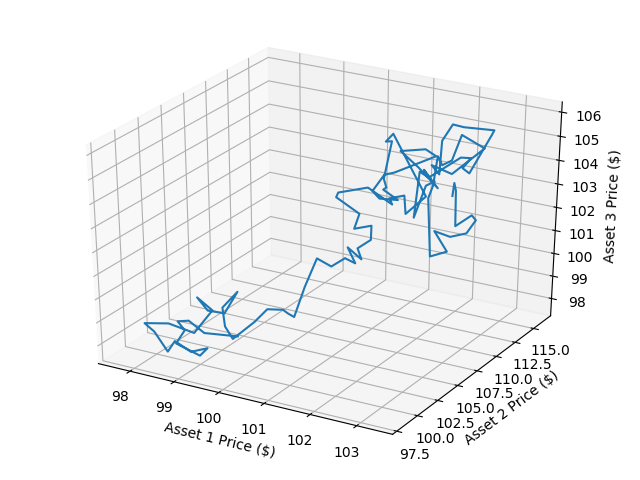
\includegraphics[width=.95\linewidth]{bin/correlated_bm_path.png}
    }
    \caption{Sample realized path of the simulation of the correlated 3-dimensional Brownian Motion process.}
    \label{fig:3d_process_viz}
\end{figure}

Figure~\ref{fig:3d_process_viz} displays a single sample simulated path from the 3-dimensional correlated Brownian Motion process.

\newpage
\subsection{Basket Option Pricing}

In this section, I price an vanilla Call and Put option, treating the correlated 3-dimensional Brownian Motion process as the underlying basket of assets on which the option is written. The sample statistics for this option are reproduced in Table~\ref{table:q3_basket_option}.

\begin{table}[!h]
    \centering
    \csvautotabular{bin/q3_basket_option.csv}
    \caption{Sample statistics of a basket option priced with a simulated 3-dimensional correlated Brownian Motion process.}
    \label{table:q3_basket_option}
\end{table}

\subsection{Exotic Basket Option Pricing}

In this section, I price an exotic option (a variant of a vanilla option, with an embedded barrier for one of the basket correlates), treating the correlated 3-dimensional Brownian Motion process as the underlying basket of assets on which the option is written. The sample statistics for this option are reproduced in Table~\ref{table:q3_exotic_option}.

\begin{table}[!h]
    \centering
    \csvautotabular{bin/q3_exotic_option_mc.csv}
    \caption{Sample statistics of an exotic basket option priced with a simulated 3-dimensional correlated Brownian Motion process.}
    \label{table:q3_exotic_option}
\end{table}

%==============================
% REFERENCES
%==============================

\newpage

\nocite{Shreve2004}
\nocite{Stefanica2011}
\nocite{Weerawarana2016}
\nocite{Florescu2019}

\printbibliography

%==============================
% APPENDIX
%==============================

\newpage

\appendix

\section{Raw Data} \label{appendix:raw_data}

    \subsection{Simple GBM Analysis} \label{appendix:raw_data:simple_gbm}

        \sisetup{round-mode=places, round-precision=5}
        \csvreader[
            longtable=c|c|cccc,
            table head=
                \toprule\bfseries Sim Count &\bfseries Eval Count &\bfseries Estimate (\$) &\bfseries Std Dev &\bfseries Std Err &\bfseries Time (s) \\ \midrule \endhead \bottomrule \endfoot,
            late after line=\\
        ]{bin/raw_simple_mc_gbm_analysis.csv}{1=\one, 2=\two, 3=\three, 4=\four, 5=\five, 6=\six}{\three & \two & \num{\one} & \num{\four} & \num{\five} & \num{\six}}
    

    \subsection{MC Method Analysis} \label{appendix:raw_data:mc_methods}

        \sisetup{round-mode=places, round-precision=5}
        \csvreader[
            longtable=l|c|cccc,
            table head=
                \toprule\bfseries Method &\bfseries Opt Type &\bfseries Estimate (\$) &\bfseries Std Dev &\bfseries Std Err &\bfseries Time (s) \\ \midrule \endhead \bottomrule \endfoot,
            late after line=\\
        ]{bin/raw_mc_methods_analysis.csv}{1=\one, 2=\two, 3=\three, 4=\four, 5=\five, 6=\six}{\one & \two & \num{\three} & \num{\four} & \num{\five} & \num{\six}}

% Resetting input path
\lstinputpath{}

\newpage
\section{Solution Source Code} \label{appendix:source}
    \subsection{Question 1 Solution} \label{appendix:source:q1}
        \lstinputlisting{question_solutions/question_1.py}

    \subsection{Question 1 Formatting Scripts}
        \subsubsection{Simple MC Analysis}
            \lstinputlisting{question_solutions/q1_format_simple_mc.py}

        \subsubsection{MC Methods Analysis}
        \lstinputlisting{question_solutions/q1_format_mc_methods.py}

    \subsection{Question 2 Solution} \label{appendix:source:q2}
        \lstinputlisting{question_solutions/question_2.py}
    
    \subsection{Question 3 Solution} \label{appendix:source:q3}
        \lstinputlisting{question_solutions/question_3.py}

\newpage
\section{\texttt{fe621} Package Code} \label{appendix:fe621}
% Setting path to parent directory
\lstinputpath{..}
    \subsection{Black-Scholes Analytical Greeks} \label{appendix:fe621:bs_greeks}
        \lstinputlisting{fe621/black_scholes/greeks.py}

%==============================
% Document End
%==============================

\end{document}
